\section{Results}
In this section, 6 experiments are presented. 5 of them are run under the simulator to test the estimation error according to several different aspects: the saccade amplitude, the noise, the depth to the camera and  the effect of robust estimation. The last experiment is run under the real system. Finally, the computational times of the algorithms are presented.
\label{sec:results}
\subsection{Simulator}
The baseline length of $53.7 \ mm$ on the torsional axis was also used in the simulator to make the comparisons easier.\\

\subsubsection{Experiment 1 - Saccade amplitudes generated with $\sigma^2 = 15 \deg $}
Figure \ref{cha5:sec1:45angle} shows the error per amplitude in degrees from 45 random saccades around all axis, simultaneously, generated in a normal distribution with variance $\sigma^2 = 15 \deg $. The lines on the graphs below represent the best fitting of the points. Table \ref{cha5:sec1:45anglet} presents the respective mean error and standard deviation. 
\begin{figure}
	\centering
	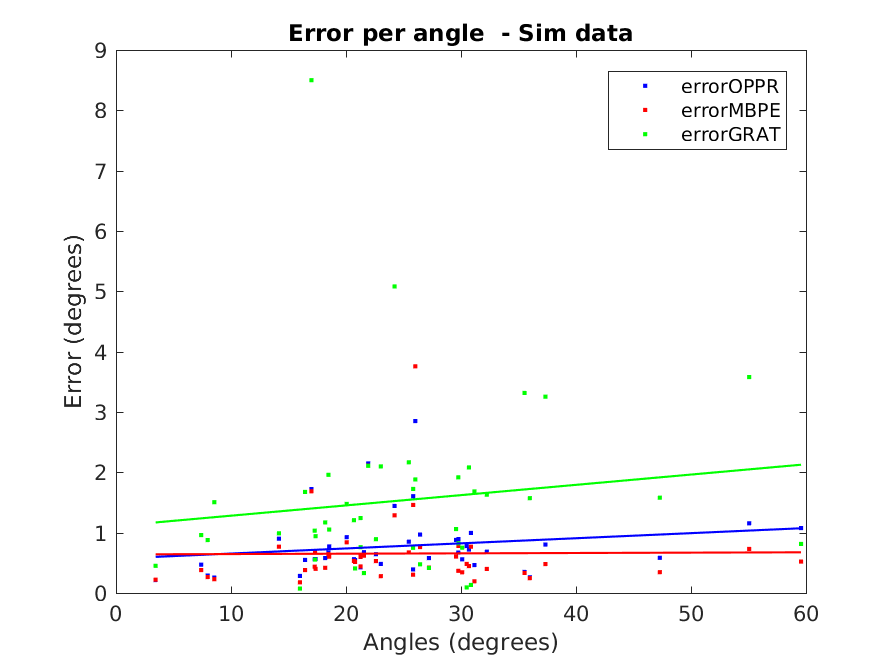
\includegraphics[width=0.5\textwidth]{images/45angle.png}
	\captionof{figure}{Experiment 1 - Error as function of amplitude (in degrees) under simulation for saccade amplitudes with $\sigma^2 = 15 \deg $}
	\label{cha5:sec1:45angle}
\end{figure}
\begin{table}
	\centering
	\begin{tabular}{| l | l | l |}
		\hline
		Method & Mean & Standard Deviation \\
		\hline
		OPPR &  $0.77 \deg$ & $0.49 \deg$ \\
		\hline
		MBPE &  $0.65 \deg$ & $0.60 \deg$ \\
		\hline
		GRAT &  $1.53 \deg$ & $1.43 \deg$ \\ 
		\hline
	\end{tabular}
	\captionof{table}{Experiment 1 mean error and standard deviation.}
	\label{cha5:sec1:45anglet}
\end{table}\\

\subsubsection{Experiment 2 - Variable noise}
To test how Gaussian noise affects the algorithms, all the same parameters as the previous section were kept and the amplitude of the saccades was set to a variance of $4 \deg$, while the added noise varies from $0$ to $100 \ px$. Figure \ref{cha5:sec1:noise} shows the error increasing with the pixel noise. 
\begin{figure}[ht]
	\centering
	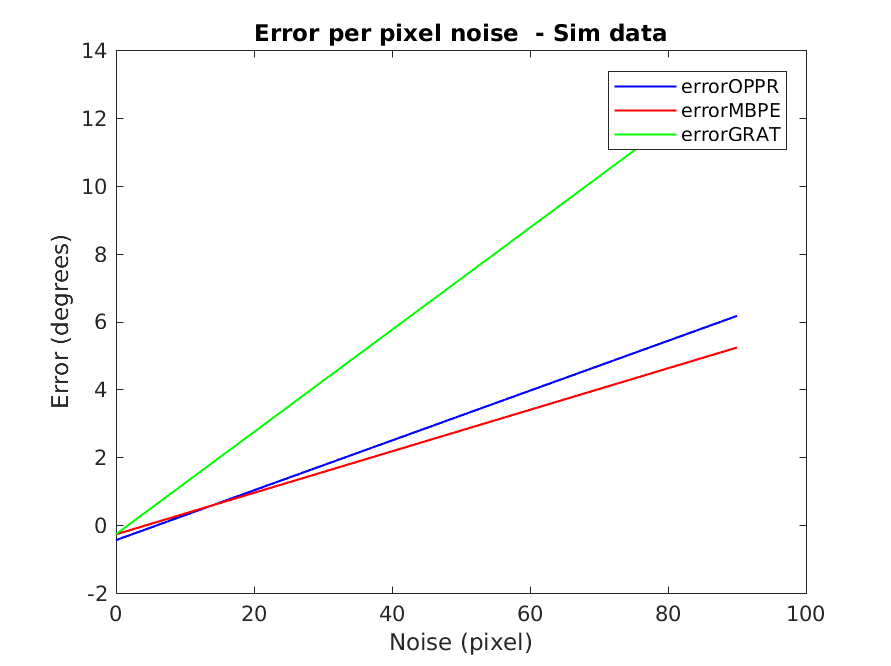
\includegraphics[width=0.5\textwidth]{images/noise.png}
	\captionof{figure}{Experiment 2 - Error (in degrees) as function of the amount of noise in the simulated image (in pixels).}
	\label{cha5:sec1:noise}
\end{figure}

\subsubsection{Experiment 3 - Variable distance}
To see how the distance from the furthest object to the camera interferes with the estimation, a simulation with the following parameters was run, with a varying distance from $5 \ cm$ to $10 \ m$. Figure \ref{cha5:sec1:depthh} exhibits the error in degrees according to the the distance to the furthest points from the camera.
\begin{figure}[ht]
	\centering
	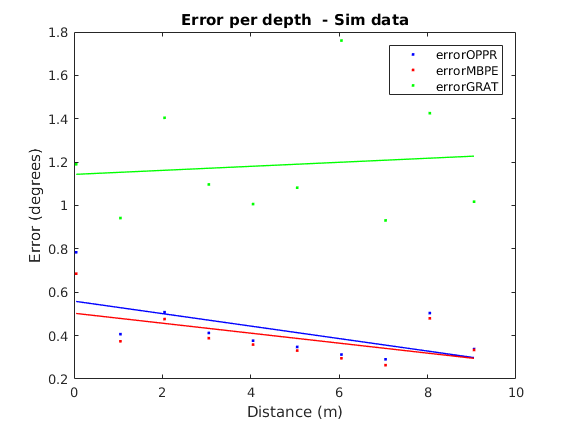
\includegraphics[width=0.5\textwidth]{images/depthh.png}
	\captionof{figure}{Experiment 3 - Error (in degrees) as function of distance to the camera in the simulated scene in meters.}
	\label{cha5:sec1:depthh}
\end{figure}	

\subsubsection{Experiment 4 - Without robust estimation}
The effect of rejecting image sections is easier to study under simulation without noise or false matches. The variance for saccade amplitude generation is now $\sigma^2 = 15 \deg $ to emphasize the effect, as bigger translations are executed. Figure \ref{cha5:sec1:withoutr} and Table \ref{cha5:sec1:withoutrt} correspond to running the algorithms without robust estimation. The amplitude of the saccades was set to a variance of $4 \deg$ in the normal distribution.\\

\begin{figure}
	\centering
	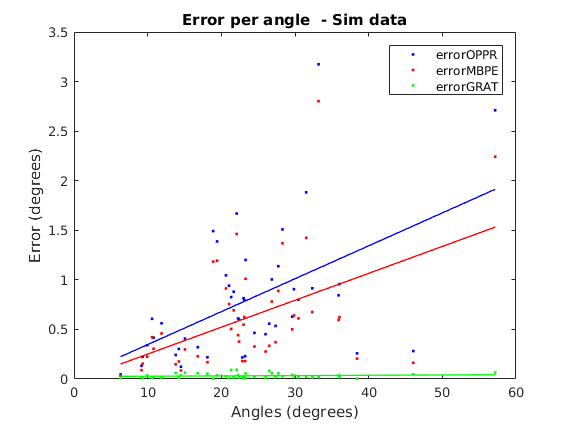
\includegraphics[width=0.5\textwidth]{images/withoutransac.png}
	\captionof{figure}{Experiment 4 - Error per saccade amplitude (in de-
		grees) under the simulation without robust estimation.}
	\label{cha5:sec1:withoutr}
\end{figure}
\begin{table}
\begin{tabular}{| l | l | l |}
	\hline
	Method & Mean & Standard Deviation \\
	\hline
	OPPR &  $0.79 \deg$ & $0.63 \deg$ \\
	\hline
	MBPE &  $0.61 \deg$ & $0.56 \deg$ \\
	\hline
	GRAT &  $0.03 \deg$ & $0.02 \deg$ \\ 
	\hline
\end{tabular}
\captionof{table}{Experiment 4 mean error and standard deviation.}
\label{cha5:sec1:withoutrt}
\end{table}

\subsubsection{Experiment 5 - With robust estimation}
Figure \ref{cha5:sec1:withr} and Table \ref{cha5:sec1:withrt} are the same as in Experiment 4 but with robust estimation.\\
\begin{figure}
	\centering
	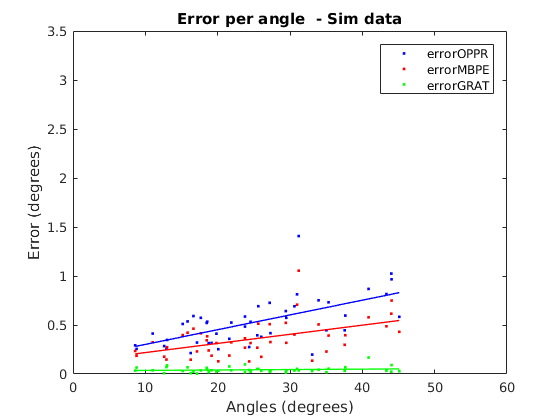
\includegraphics[width=0.5\textwidth]{images/withransac.png}
	\captionof{figure}{Experiment 5 - Error per saccade amplitude (in de-
		grees) under the simulation with robust estimation.}
	\label{cha5:sec1:withr}
\end{figure}
\begin{table}
\begin{tabular}{| l | l | l |}
	\hline
	Method & Mean & Standard Deviation \\
	\hline
	OPPR &  $0.53 \deg$ & $0.24 \deg$ \\
	\hline
	MBPE &  $0.36 \deg$ & $0.18 \deg$ \\
	\hline
	GRAT &  $0.04 \deg$ & $0.03 \deg$ \\ 
	\hline
\end{tabular}
\captionof{table}{Experiment 5 mean error and standard deviation..}
\label{cha5:sec1:withrt}
\end{table}

\subsection{Real system}
To test the algorithms under the real system, 10 images of a scene, with the setup mentioned on \ref{cha4:sec3:eyescheme}, were took with and without a chessboard at the same time as the IMU collected the current orientation of the eye prototype, for each experiment. Joining the images/orientations with each other made up to 45 different saccades. 
\subsubsection{Experiment 6 - Rotation estimation error}
Figure \ref{cha5:sec1:r1angle} presents the error per saccade amplitude on the real system in degrees for the camera, and Figure \ref{cha5:sec1:r1angleimu} shows the same for the IMU. Table \ref{cha5:sec1:r1anglet} displays the corresponding mean error and standard deviation for each method and for the IMU. The lines on the graphs below represent the best fitting of the points.

\begin{figure}
\centering
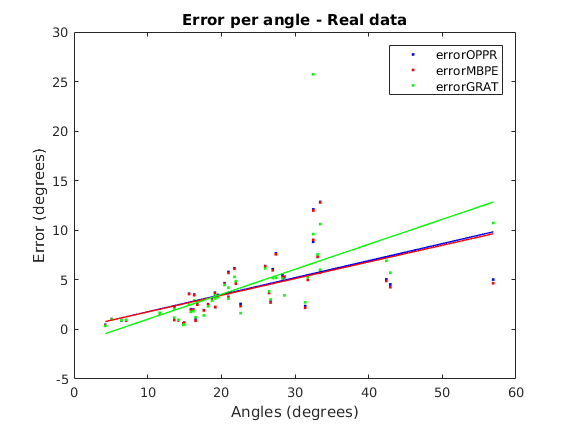
\includegraphics[width=0.5\textwidth]{images/r1angle.png}
\captionof{figure}{Experiment 6 - Error per saccade amplitude (in degrees) under the real system for the camera estimation.}
\label{cha5:sec1:r1angle}
\end{figure}
\begin{figure}
\centering
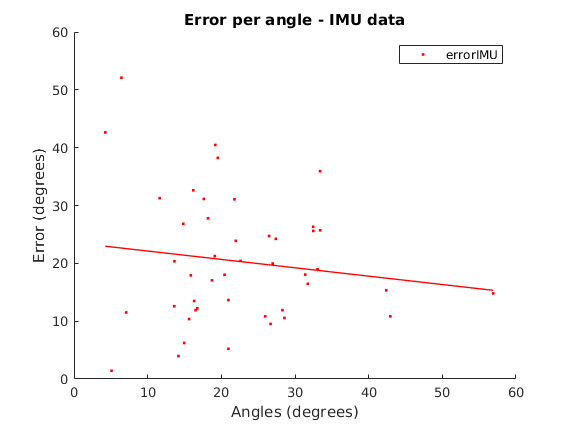
\includegraphics[width=0.5\textwidth]{images/r1angleimu.png}
\captionof{figure}{Experiment 6 - Error per saccade amplitude (in degrees) under the real system for the IMU estimation.}
\label{cha5:sec1:r1angleimu}
\end{figure}

\begin{table}[ht]
	\centering
\begin{tabular}{| l | l | l |}
	\hline
	Method & Mean & Standard Dev. \\
	\hline
	OPPR &  $3.90 \deg$ & $2.75 \deg$ \\
	\hline
	MBPE &  $3.83 \deg$ & $2.75 \deg$ \\
	\hline
	GRAT &  $4.13 \deg$ & $4.09 \deg$ \\ 
	\hline
	IMU &  $20.34 \deg$ & $10.85 \deg$ \\ 
	\hline
	IMU w/o vertical axis &  $11.79 \deg$ & $3.57 \deg$ \\ 
	\hline
\end{tabular}
\captionof{table}{Experiment 6 mean error and standard deviation.}
\label{cha5:sec1:r1anglet}
\end{table}

\begin{figure}[ht]
	\centering
	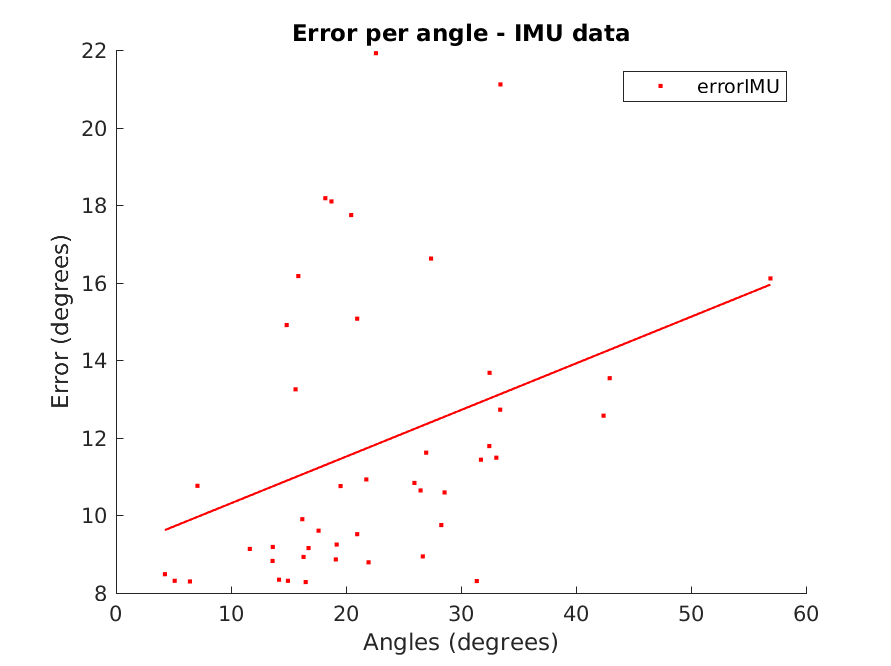
\includegraphics[width=0.5\textwidth]{images/imuerrorissue.png}
	\captionof{figure}{Experiment 6 but only visualizing the error on the horizontal and torsional axis.}
	\label{cha5:sec1:imuerrorissue}
\end{figure}

\subsubsection{Computational time}
When using the created C++ library, the computational times seen on Table \ref{cha5:sec1:speed} were obtained for each of the processes that have to be executed to estimate the eye prototype's orientation and for the IMU estimation.

\begin{table}[ht]
	\centering
	\begin{tabular}{| l | l | l |}
		\hline
		Process & Time \\
		\hline
		Image Capture & $120 \ ms$  \\
		\hline
		Undistort + Find Keypoints &   $421 \ ms$ \\
		\hline
		Find Matches & $16 \ ms$ \\ 
		\hline
		Robust Estimation & $10 \ ms$ \\ 
		\hline
		OPPR & $13\mathrm{e}{-2} \ ms$ \\ 
		\hline
		MBPE & $212 \ ms$ \\ 
		\hline
		GRAT & $51 \ ms$ \\ 
		\hline
		IMU Estimation &  $40\mathrm{e}{-4} \ ms$ \\ 
		\hline
	\end{tabular}
	\captionof{table}{Computational time for each of the necessary processes to estimate the orientation of the eye prototype in C++.}
	\label{cha5:sec1:speed}
\end{table}

\section{Discussion}

In Table \ref{cha5:sec1:45anglet} and Figure \ref{cha5:sec1:45angle} (Experiment 1), the best two methods are OPPR and MBPE. MBPE seems to be the best method in this case when run under simulation. As the saccade amplitude increases, OPPR becomes worst This may be due to the fact that for a bigger saccade, the associated translation creates a larger effect that is not counter acted when using this algorithm. As for GRAT, it performs worst than the other algorithms, because the baseline length is small, the fundamental matrix expressed in (\ref{deewfwfe}), will have values very close to zero, that during intermediate calculus in the minimization can reduce the accuracy of the estimation. Other reason could be that, because the depth, $\lambda$, is not being estimated, opposite to MBPE, the leeway to estimate the rotation is reduced, ending up with a poorer guess.

In Experiment 2, it can be seen that GRAT is more sensitive to noise than the others.

The further away the points are, the more approximate to a pure rotation the movement becomes. By looking at Experiment 3, OPPR and MBPE, improve with distance, probably due to rejecting image sections. GRAT makes use of translation to get a good estimation, so it doesn't really gain anything from distance, except for a better initialization given by OPPR.

RANSAC+OPPR for robust estimation yield point matches that are more approximate to a pure rotation. By the results of Experiment 4, it's possible to see that it has slightly improved by using robust estimation for the methods OPPR and MBPE. For the former, this was very expected, as it is most accurate when dealing with pure rotations, as for MBPE by taking OPPR as an initialization parameter, it is normal to also have its results improved. GRAT, however, has a really small error now compared to the results in Experiment 1, which probably indicates that it is extremely sensitive to Gaussian noise in the images, that is not present here. This in fact makes sense, as this algorithm uses pixel coordinates directly to estimate the rotation.

Experiment 6 for the camera estimation (Figure \ref{cha5:sec1:r1angle}), done under the real system, performed similarly to Experiment 1 as OPPR and MBPE keep being better than GRAT. Experiment 6's best mean error for the camera is $3.83 \deg $ from MBPE with a standard deviation of $2.75 \deg$. This error is probably due to noise in the image or even false matches that were not filtered out in the robust estimation. As it is real data, there is always noise associated and imposing stricter parameters  for RANSAC will eventually not yield enough point matches to work with. 
As for the IMU estimation results (Figure \ref{cha5:sec1:r1angleimu}), it manifests a huge error in relation to the camera. Besides that, this error doesn't seem to have a pattern like the camera's, where the error increases with the saccade amplitude. This outcome may be caused by unstable measurements during the experiment, as the IMU needs to stabilize its position for some time until it gives a correct orientation. It could also be justified by the drift specially when associated to rotations around the vertical axis (as it cannot use the force of gravity for the measurements). This last motivation can be backed up by Figure \ref{cha5:sec1:imuerrorissue}, that shows the same as Figure \ref{cha5:sec1:r1angleimu} without the rotation estimation around the vertical axis, presenting half the error as previously and an increasing pattern.

Regarding the computational error, obviously, the IMU takes much less time estimating the orientation than the camera. For the quickest algorithm, OPPR, the total amount of time taken is $567 \ ms$. 

Having said that, it's possible to make the following remarks summarizing each estimation method.

\begin{itemize}
	\item OPPR is the fastest and the most light-weight of the camera estimation methods. Because it ignores the translation associated to the eye prototype rotations, it performs better when the movement is closer to pure rotations. If the scenery is very far way, the algorithm improves. Using RANSAC+OPPR to filter out point matches also refines the estimation.
	
	\item MBPE seemed to be the best camera algorithm out of all the Experiments. However, because it has to estimate both the three Euler angles and depth, $\lambda$, for each point match, a total of ($2+n$) parameters, it is the one that takes the longest. It improves when OPPR improves, as it highly depends on the initialization.
	
	\item GRAT did the worst in the Experiments and proved to be very sensitive to pixel noise in the image. It does better when associated to bigger saccade amplitudes, as they have more translation associated. It has a big downside, which is not working for pure rotations, as mentioned on section \ref{fjeopfe}.
	
	\item IMU estimation is the fastest method but the error is much higher than in the camera algorithms, most probably due to rotation around the vertical axis.	
	
\end{itemize}

The most accurate method is the Minimization of the back projection error (MBPE). 
